\uuid{r0au}
\chapitre{Fonction de plusieurs variables}
\niveau{L2}
\module{Analyse}
\sousChapitre{Autre}
\titre{Courbes de niveau}
\theme{fonctions de plusieurs variables}
\auteur{}
\datecreate{2023-03-01}
\organisation{AMSCC}
\difficulte{}
\contenu{

	
		A chaque fonction définie ci-dessous (1-6), associer ses courbes de niveaux (A-F).
\begin{enumerate}
	\item \question{  $f(x,y) = \sin(xy)$ }
	\reponse{1-B : la fonction est périodique en $x$ et en $y$ ; $f$ ne change pas quand on échange $x$ et $y$, i.e. le graphe est symétrique par rapport au plan d’équation $y = x$ ; $f (0, y) = f (x,0) = 0$.}
	\item \question{  $f(x,y) = \sin(x-y)$ }
	\reponse{2-A : la fonction est périodique en $x$ et en $y$ ; $f$ est constante si $y = x +k$ (lignes de niveau parallèles à la droite d'équation $y=x$}
	\item \question{ $f(x,y) = (1-x^2)(1-y^2)$ }
	\reponse{3-F : $f (\pm1, y) = f (x,\pm1) = 0$ ; la trace dans le plan $xz$ est $z = 1-x^2$ et dans le plan $yz$ est $z = 1-y^2$.}
	\item \question{ $f(x,y) = \frac{x-y}{1+x^2+y^2}$ }
	\reponse{4-E : $f (x,x) = 0$ ; $f (x, y) > 0$ si $x > y$ ; $f (x, y) < 0$ si $x < y$.}
	\item \question{ $f(x,y) = e^x \cos(y)$ }
	\reponse{5-D : la fonction est périodique en $y$ ;}
	\item \question{ $f(x,y) = \sin(x)-\sin(y)$ }
	\reponse{6-C : la fonction est périodique en $x$ et en $y$.}
\end{enumerate}

\begin{minipage}{0.5\textwidth}
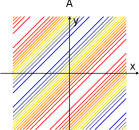
\includegraphics[]{pdf/r0au-tikz-1}
\end{minipage}
\hfill
\begin{minipage}{0.5\textwidth}
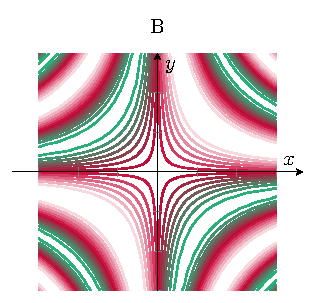
\includegraphics[]{pdf/r0au-tikz-2}
\end{minipage}

\begin{minipage}{0.5\textwidth}
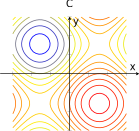
\includegraphics[]{pdf/r0au-tikz-3}
\end{minipage}
\hfill
\begin{minipage}{0.5\textwidth}
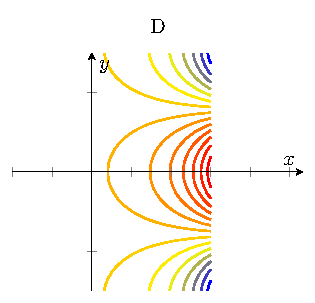
\includegraphics[]{pdf/r0au-tikz-4}
\end{minipage}

\begin{minipage}{0.5\textwidth}
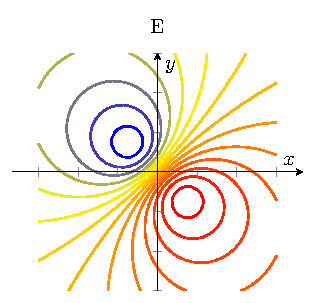
\includegraphics[]{pdf/r0au-tikz-5}
\end{minipage}
\hfill
\begin{minipage}{0.5\textwidth}
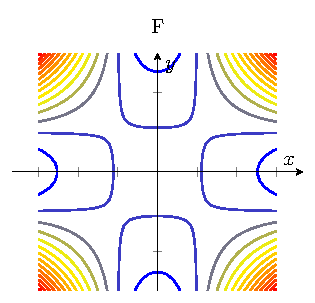
\includegraphics[]{pdf/r0au-tikz-6}
\end{minipage}

}
